\titleformat{\chapter}[display]
  {\normalfont\Large\bfseries}{\centering Tuần 9}{10pt}{\centering\Huge\bfseries}
  
\chapter{Nhập Môn Cơ Học Giải Tích}

\section{Liên kết động học} 
\label{sec_9:Kinematic_link}

Phần lớn các học sinh bắt đầu khảo sát các liên kết chuyển động dựa trên những trực giác mơ hồ, các nhận định cảm tính các phương pháp đổi hệ quy chiếu.
Thoạt đầu, sự thông minh và sự nhạy bén về khả năng tưởng tượng hình học giúp cho nhiều học sinh nhanh chóng giải quyết được vấn đề một cách hiệu quả.
Song, với các cơ hệ phức tạp bao gồm nhiều liên kết chuyển động, các vật chuyển động trong không gian 3 chiều, những quan sát cảm tính thường xuyên mang đến những kết luận sai.
Các lý thuyết về liên kết động học, ứng dụng giải tích trong khảo sát các liên hệ về tọa độ, lực, gia tốc mang đến sự chặt chẽ.
Không những giúp cho chúng ta có một lời giải chắc chắn, các lý thuyết về liên kết là một đường lối chuẩn mực cho lời giải các bài toán cơ học, giúp không chỉ con người với trí khả năng tư duy trừu tượng sâu sắc, mà ngay cả các hệ thống máy tính, lập trình cũng có thể tự thiết lập được các phương trình vi phân mô tả chuyển động.

Trong mục này, chúng ta sẽ khảo sát các liên kết chuyển động dựa trên hệ thống các bậc tự do, hệ tọa độ suy rộng, phân biệt các loại liên kết và ứng dụng lý thuyết giải tích trong tính toán các vận tốc, gia tốc trong hệ cơ học.


\subsection{Bậc tự do}

Tập hợp các thông số \textbf{đủ} để xác định được vị trí của cơ hệ trong một hệ quy chiếu xác định, được gọi là các tọa độ suy rộng của cơ hệ.\\
Các tọa độ suy rộng được kí hiệu là $q_1, q_2, \ldots, q_m$. Các tọa độ suy rộng có thể là các tọa độ Đề các của các chất điểm thuộc cơ hệ, có thể là góc quay, các tọa độ cong\ldots\\
Bản chất vật lý của tọa độ suy rộng là bất kỳ, do đó thứ nguyên của nó có thể không phải là độ dài như tọa độ Đề các.\footnote{Dựa theo quyển sách "Bài tập Cơ học Tập 2: Động lực học" của giáo sư Đỗ Sanh.}\\
Vị trí của cơ hệ được xác định nhờ tọa độ suy rộng, nên các tọa độ Decartes của các chất điểm của cơ hệ có thể biểu diễn qua các tọa độ suy rộng:
\begin{align*}
    x_k &= x_k(t, q_1, q_2, \ldots, q_m)\\
    y_k &= y_k(t, q_1, q_2, \ldots, q_m)\\
    z_k &= z_k(t, q_1, q_2, \ldots, q_m)
\end{align*}
Hoặc viết ở dạng rút gọn:
\begin{equation*}
    \mathbf{r_k} = \mathbf{r_k}(t, q_1, q_2, \ldots, q_m)
\end{equation*}
Ta xét trường hợp con lắc đôi, để xác định vị trí của con lắc ta có những tọa độ sau: (ĐANG CẬP NHẬT HÌNH MINH HỌA)
\begin{align*}
    (x_A, y_A, x_B, y_B)\\
    (\theta, \phi)
\end{align*}
Nhận thấy trong hai tập hợp nêu trên, tập hợp đầu tiên các thông số không độc lập với nhau, quả thực vậy đối với tập hợp thứ nhất:
\begin{equation*}
    {x_A}^2+{y_B}^2 = {l_1}^2; {(x_B - x_A)}^2+{(y_B - y_A)}^2 = {l_2}^2
\end{equation*}
với tập hợp thứ hai, các tọa độ đề các của các chất điểm của cơ hệ được biểu diễn bằng các hệ thức sau:
\begin{align*}
    x_A &= OA\cos{\theta}, \\
    y_A &= OA\sin{\theta}, \\
    x_B &= OA\cos{\theta} + AB\cos{\phi}, \\
    y_B &= OA\sin{\theta} + AB\sin{\phi}.
\end{align*}
Vậy tập hợp $(\theta, \phi)$ là các tọa độ suy rộng \textbf{đủ} của hệ con lắc. Còn $(x_A, y_A, x_B, y_B)$ là các tọa độ suy rộng \textbf{dư}.

\subsection{Liên kết Holonom và liên kết phi Holonom}

Một phương trình liên kết động học thông thường sẽ có dạng
\begin{equation}
    f(\mathbf{q}, \mathbf{\dot{q}}, t) = 0.
\end{equation}
Với $\mathbf{q} = [q_1,q_2,\ldots,q_n]$ và $\mathbf{\dot{q}} = [\dot{q}_1,\dot{q}_2,\ldots,\dot{q}_n]$ là các tọa độ, tọa độ suy rộng của cơ hệ và đạo hàm bậc nhất (vận tốc) của chúng.

Từ phương trình liên kết trên, ta có thể phân loại các cơ hệ thành một số loại như sau \footnote{Dựa theo quyển sách "Cơ học giải tích" của giáo sư Nguyễn Quang Đạo.}:
\begin{itemize}
    \item \textbf{Liên kết holonom (honomic)}, hay còn được gọi là \textbf{liên kết hình học}, \textbf{liên kết hữu hạn}, là các liên hệ không phụ thuộc vào các đạo hàm bậc nhất của các tọa độ, tức là
    \begin{equation*}
        f(\mathbf{q}, t) = 0.
    \end{equation*}
    và ngược lại là \textbf{ liên kết phi holonom (nonholonomic)}.
    \item \textbf{Liên kết scleronom (scleronomous)}, hay còn được gọi là \textbf{liên kết dừng}, là các liên kết không phụ thuộc tường minh vào thời gian (tức là $\partial \mathbf{q} / t = 0$), ngược lại với nó là \textbf{liên kết Rheonom (Rheonomous)}, hay còn được gọi là \textbf{liên kết không dừng}.
    \item Liên kết giữ và không giữ\ldots %sẽ được bổ sung sau
\end{itemize}
Trong các ứng dụng kỹ thuật, các cánh tay robot, các cơ cấu tay chi tiết máy thường là các liên kết holonom. 
Còn các liên kết phi holonom thường xuất hiện trong các hệ mobile robot, máy bay, drone,\ldots 
Để xác định tọa độ qua các liên kết holonom, ta chỉ cần xác định thông qua các tính chất hình học. 
Trong khi đó, với các hệ liên kết phi holonom, việc xác định tọa độ của các vật thể trở nên tương đối phức tạp, đòi hỏi ta phải ứng dụng các kỹ thuật định vị ngoài cơ học như sử dụng các cảm biến, sóng điện từ, radar,\ldots 
Trong tài liệu này, ta sẽ chỉ tập trung vào lĩnh vực cơ lý thuyết, vì vậy, cụ thể ta sẽ chỉ phân tích về các cơ hệ có các liên kết holonom.

\subsection{Ứng dụng đạo hàm toàn phần và ma trận Jacobian trong tính toán vận tốc, gia tốc các điểm của cơ hệ Holonom}

Giả sử trong một cơ hệ có $n$ bậc tự do với các tọa độ suy rộng tương ứng là $\mathbf{q} = [q_1,q_2,\ldots,q_n]$. Với một tọa độ bất kỳ nào đó có liên kết phụ thuộc vào các tọa độ suy rộng kia theo dạng có thể tách biến được:
\begin{equation*}
    x = f(\mathbf{q})
\end{equation*}
Ta sẽ có thể tìm vận tốc, tức là đạo hàm bậc nhất của $x$ theo thời gian $t$ theo công thức của đạo hàm toàn phần:
\begin{equation}
    x = \dfrac{\partial f(\mathbf{q})}{\partial \mathbf{q}} \mathbf{\dot{q}} + \dfrac{\partial f (\mathbf{q})}{\partial t}.
\end{equation}
Đối với các liên kết Holonom \(\partial f/ \partial t = 0\), nên 
\begin{equation}
    x = \dfrac{\partial f(\mathbf{q})}{\partial \mathbf{q}} \mathbf{\dot{q}}.
\end{equation}
\subsection{Lực bị động trong bài toán liên kết Holonom}


\section{Cơ học Lagrange}

\subsection{Nguyên lý tác dụng tối thiểu}

\subsection{Phương trình Lagrange loại II}

\subsection{Phương trình Lagrange loại I}

\subsection{Động lượng suy rộng}

\subsection{Định lý Noether}

% Continuous symmetry

% Bài tập ví dụ: Xác định phương trình vi phân mô tả chuyển động của con lắc kép.

\subsection{Giải phương trình chuyển động bằng phương pháp Runge-Kutta 4}

\subsection{Tính toán lực bị động dựa trên phương trình Lagrange loại 2}

\section{Các lý thuyết cơ học giải tích khác}

\subsection{Cơ học Hamilton}

\subsection{Nguyên lý Gauss về liên kết tối thiểu}

\subsection{Phương trình Appell cho cơ hệ phi Holonom}


\section{Bài tập}

\subsection*{Chuyển động liên kết}

\textbf{Bài 9.1:} Va chạm vuông vắn (Hướng tới VPhO 43)

Hai thanh thẳng đồng chất, cứng, dài \(l\) được nối với nhau bằng một bản lề ở đầu thanh. 
Các đầu của hai thanh cứng này trượt trên khung hình vuông, đặt cố định trong mặt phẳng nằm ngang, có độ dài cạnh là \(L\) (với \(\frac{\sqrt{3}}{2}l<L<2l\) ). 
Ta lần lượt gọi 3 điểm đầu các thanh là \(A\), \(B\), \(C\) (như hình \ref{fig:9_P1}). Góc tạo bởi thanh \(AB\) và cạnh khung hình vuông có chứa đầu \(A\) là \(\theta\). Bỏ qua ma sát ở khung vuông, thanh trượt và các bản lề.

\begin{figure}[!h]
    \centering
    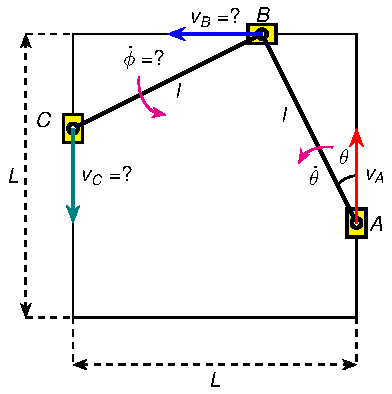
\includegraphics[width=0.5\textwidth]{Tuan9/Figures/Fig_P9_1/Fig_P9_1.pdf}
    \caption{Khung và các thanh quay.}
    \label{fig:9_P1}
\end{figure}

\begin{enumerate}
    \item Tìm vận tốc của \(B\), \(C\) và vận tốc góc của thanh \(BC\) theo \(\theta\) và vận tốc góc \(\dot{\theta}\) của thanh \(AB\).
    \item Tại một thời điểm \(A\) có vận tốc là \(v\), gia tốc là \(a\), góc \(\theta=\theta_0\) thì gia tốc của \(B\) là bao nhiêu?
\end{enumerate}

\textbf{Bài 9.2:} Cơ cấu tay quay con trượt (VPhO 2020)

Một cơ cấu cơ khí thanh truyền tay quay (như hình \ref{fig:9_P2}). 
Tay quay \(OA\) có chiều dài \(r\) và quay đều với vận tốc góc \(\omega\) quanh trục quay cố định \(O\), chiều quay cùng chiều kim đồng hồ. 
Thanh truyền \(AB\) có chiều dài \(l\) và điểm \(B\) ở đầu thanh gắn với con trượt luôn chuyển động thẳng trên một rãnh nằm ngang. 
Xét trong hệ quy chiếu gắn với mặt đất, ta cần xác định các đặc trưng động học của thanh \(AB\).

\begin{figure}[!h]
    \centering
    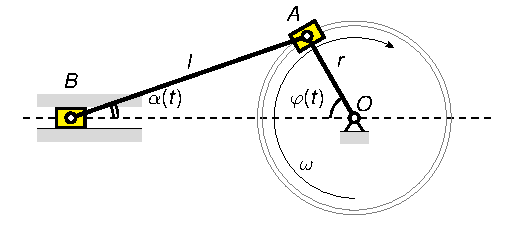
\includegraphics[width=0.8\textwidth]{Tuan9/Figures/Fig_P9_2/Fig_P9_2.pdf}
    \caption{Cơ cấu tay quay - con trượt.}
    \label{fig:9_P2}
\end{figure}

\begin{enumerate}
	\item Tại thời điểm tay quay \(OA\) tới vị trí góc \(\widehat{OAB}= \frac{\pi}{2}\), hãy xác định:
        \subitem a, Vận tốc \(\mathbf{v_B}\) của đầu \(B\).
        \subitem b, Vận tốc góc \(\omega_{AB}\) của thanh \(AB\).
        \subitem c, Gia tốc \(\vec{a}_B\) của đầu \(B\) và gia tốc góc \(\gamma_{AB}\) của thanh \(AB\).
        
Áp dụng bằng số tính \(v_B\), \(\omega_{AB}\), \(a_B\), \(\gamma_{AB}\) với các giá trị \(r = \SI{10}{cm}\), \(\omega = \SI{5}{rad/s}\), \(l = \SI{30}{cm}\).
    \item Khi tay quay \(OA\) tới vị trí ứng với góc \(\varphi = \widehat{BOA} = \dfrac{\pi}{2}\), hãy xác định: 
        \subitem a, Gia tốc \(\vec{a}_B\) của đầu \(B\).
        \subitem b, Gia tốc góc \(\gamma_{AB}\) của thanh \(AB\).
        \subitem c, Ví trí \(M\) và \(N\) trên thanh \(AB\) tương ứng với điểm có gia tốc lớn nhất và gia tốc nhỏ nhất. Xác định gia tốc của các điểm đó.
    \item Khảo sát chuyển động của đầu \(B\) của thanh $AB$ theo thời gian \(t\):
        \subitem a, Viết phương trình vận tốc \(v_B\) của điểm $B$ theo thời gian \(t\) với \(0 \le t \le \frac{2 \pi}{\omega}\), chọn gốc thời gian \(t = 0\) khi \(\varphi (0) = 0\).
        \subitem b, Cơ cấu cơ khí trên cần có điều kiện gì để con trượt dao động điều hòa?
\end{enumerate}

\subsection*{Cơ học Lagrange}


\section{Lời giải}

\textbf{Bài 9.1:} 

\textbf{1.} Các tọa độ và vận tốc lần lượt được biểu diễn theo $\theta$ và $\dot{\theta}$ dưới dạng:
\begin{align*}
    x_A &= L - l \cos \theta \Rightarrow v_A= \dot{\theta} l \sin \theta. \\
    x_B &= l \sin \theta \Rightarrow v_B = \dot{\theta} l \cos \theta. \\
    \varphi &= \arccos \left( \dfrac{L - l \sin \theta}{l} \right) \Rightarrow \dot{\varphi} = \dot{\theta} \dfrac{l \cos \theta}{\sqrt{l^2 - \left( L - l \sin \theta \right)^2}}. \\
    x_C &= \sqrt{l^2 - \left( L - l \sin \theta \right)^2} \Rightarrow v_C = \dot{\theta} \dfrac{(L-l \sin \theta) l \cos \theta}{\sqrt{l^2 - \left( L - l \sin \theta \right)^2}}.
\end{align*}

\textbf{2.} Tại thời điểm $v_A=v$ và $a_A=a$, ta có thể tìm lại $\dot{\theta}$ và $\ddot{\theta}$ theo các bước:
\begin{equation} \label{eq1_rectangle_collision}
    v=\dot{\theta} l \sin \theta \Rightarrow \dot{\theta}= \dfrac{v}{l \sin \theta}.
\end{equation}
Đạo hàm $v=\dot{\theta} l \sin \theta$ theo thời gian, ta được
\begin{equation} \label{eq2_rectangle_collision}
    a = \ddot{\theta} l \sin \theta + \dot{\theta}^2 l \cos \theta = \ddot{\theta} l \sin \theta + \dfrac{v^2}{l} \dfrac{\cos \theta}{\sin^2 \theta} \Rightarrow \ddot{\theta}= \dfrac{a}{l \sin \theta} - \dfrac{v^2}{l^2} \dfrac{\cos \theta}{\sin^3 \theta}.
\end{equation}
Đạo hàm biểu thức $v_B$ ta tìm được ở phần \textbf{a,} theo thời gian
\begin{equation} \label{eq3_rectangle_collision}
    a_B = \ddot{\theta} l \cos \theta - \dot{\theta}^2 l \sin \theta.
\end{equation}
Thế $\dot{\theta}$ và $\ddot{\theta}$ từ phương trình trên vào, thay $\theta=\theta_0$, ta tìm được gia tốc của $B$
\begin{equation} \label{eq4_rectangle_collision}
    a_B = \dfrac{1}{\tan \theta_0} a - \dfrac{v^2}{l \sin^3 \theta_0}.
\end{equation}


\textbf{Bài 9.2:}
